\documentclass[letter]{bioinfo}
\copyrightyear{2018} \pubyear{2018}

\access{Advance Access Publication Date: Day Month Year}
\appnotes{Review article}
\graphicspath{{../figures/}}

\newcommand{\comment}[1]{\textcolor{red}{#1}}
\newcommand{\todo}[1]{\colorbox{yellow}{\parbox{1\linewidth}{#1}}}

\begin{document}
\firstpage{1}

\subtitle{Review}

\title[short Title]{Cardioinformatics: the unmet need to pioneer an emerging field at the nexus of bioinformatics and cardiology}
\author[Sample \textit{et~al}.]{Bohdan B. Khomtchouk\,$^{\text{\sfb 1,}*}$, Diem-Trang Tran\,$^{\text{\sfb 2}}$, Themistocles L. Assimes\,$^{\text{\sfb 3, 4}}$ and Or Gozani\,$^{\text{\sfb 1}}$}
\address{$^{\text{\sf 1}}$Department of Biology, Stanford University, Stanford, CA, USA \\
$^{\text{\sf 2}}$School of Computing, University of Utah, Salt Lake City, UT, USA \\
$^{\text{\sf 3}}$Department of Medicine, Division of Cardiovascular Medicine, Stanford University, Stanford, CA, USA \\
$^{\text{\sf 4}}$VA Palo Alto Health Care System, Palo Alto, CA, USA
}

\corresp{$^\ast$To whom correspondence should be addressed.}

\history{Received on XXXXX; revised on XXXXX; accepted on XXXXX}

\editor{Associate Editor: XXXXXXX}

\abstract{\textbf{Motivation:} Text Text Text Text Text Text Text Text Text Text Text Text Text
Text Text Text Text Text Text Text Text Text Text Text Text Text Text Text Text Text Text Text
Text Text Text Text Text Text Text Text Text Text Text Text Text Text Text Text Text Text Text
Text Text Text Text Text Text
Text Text Text Text Text.\\
\textbf{Results:} Text  Text Text Text Text Text Text Text Text Text  Text Text Text Text Text
Text Text Text Text Text Text Text Text Text Text Text Text Text  Text Text Text Text Text Text\\
\textbf{Availability:} Text  Text Text Text Text Text Text Text Text Text  Text Text Text Text
Text Text Text Text Text Text Text Text Text Text Text Text Text Text  Text\\
\textbf{Contact:} \href{bohdan@stanford.edu}{bohdan@stanford.edu}\\
\textbf{Supplementary information:} Supplementary data are available at \textit{Briefings in Bioinformatics}
online.}

\maketitle

\section{The current status of bioinformatics in cardiovascular  research}
\begin{figure}
	\centering
	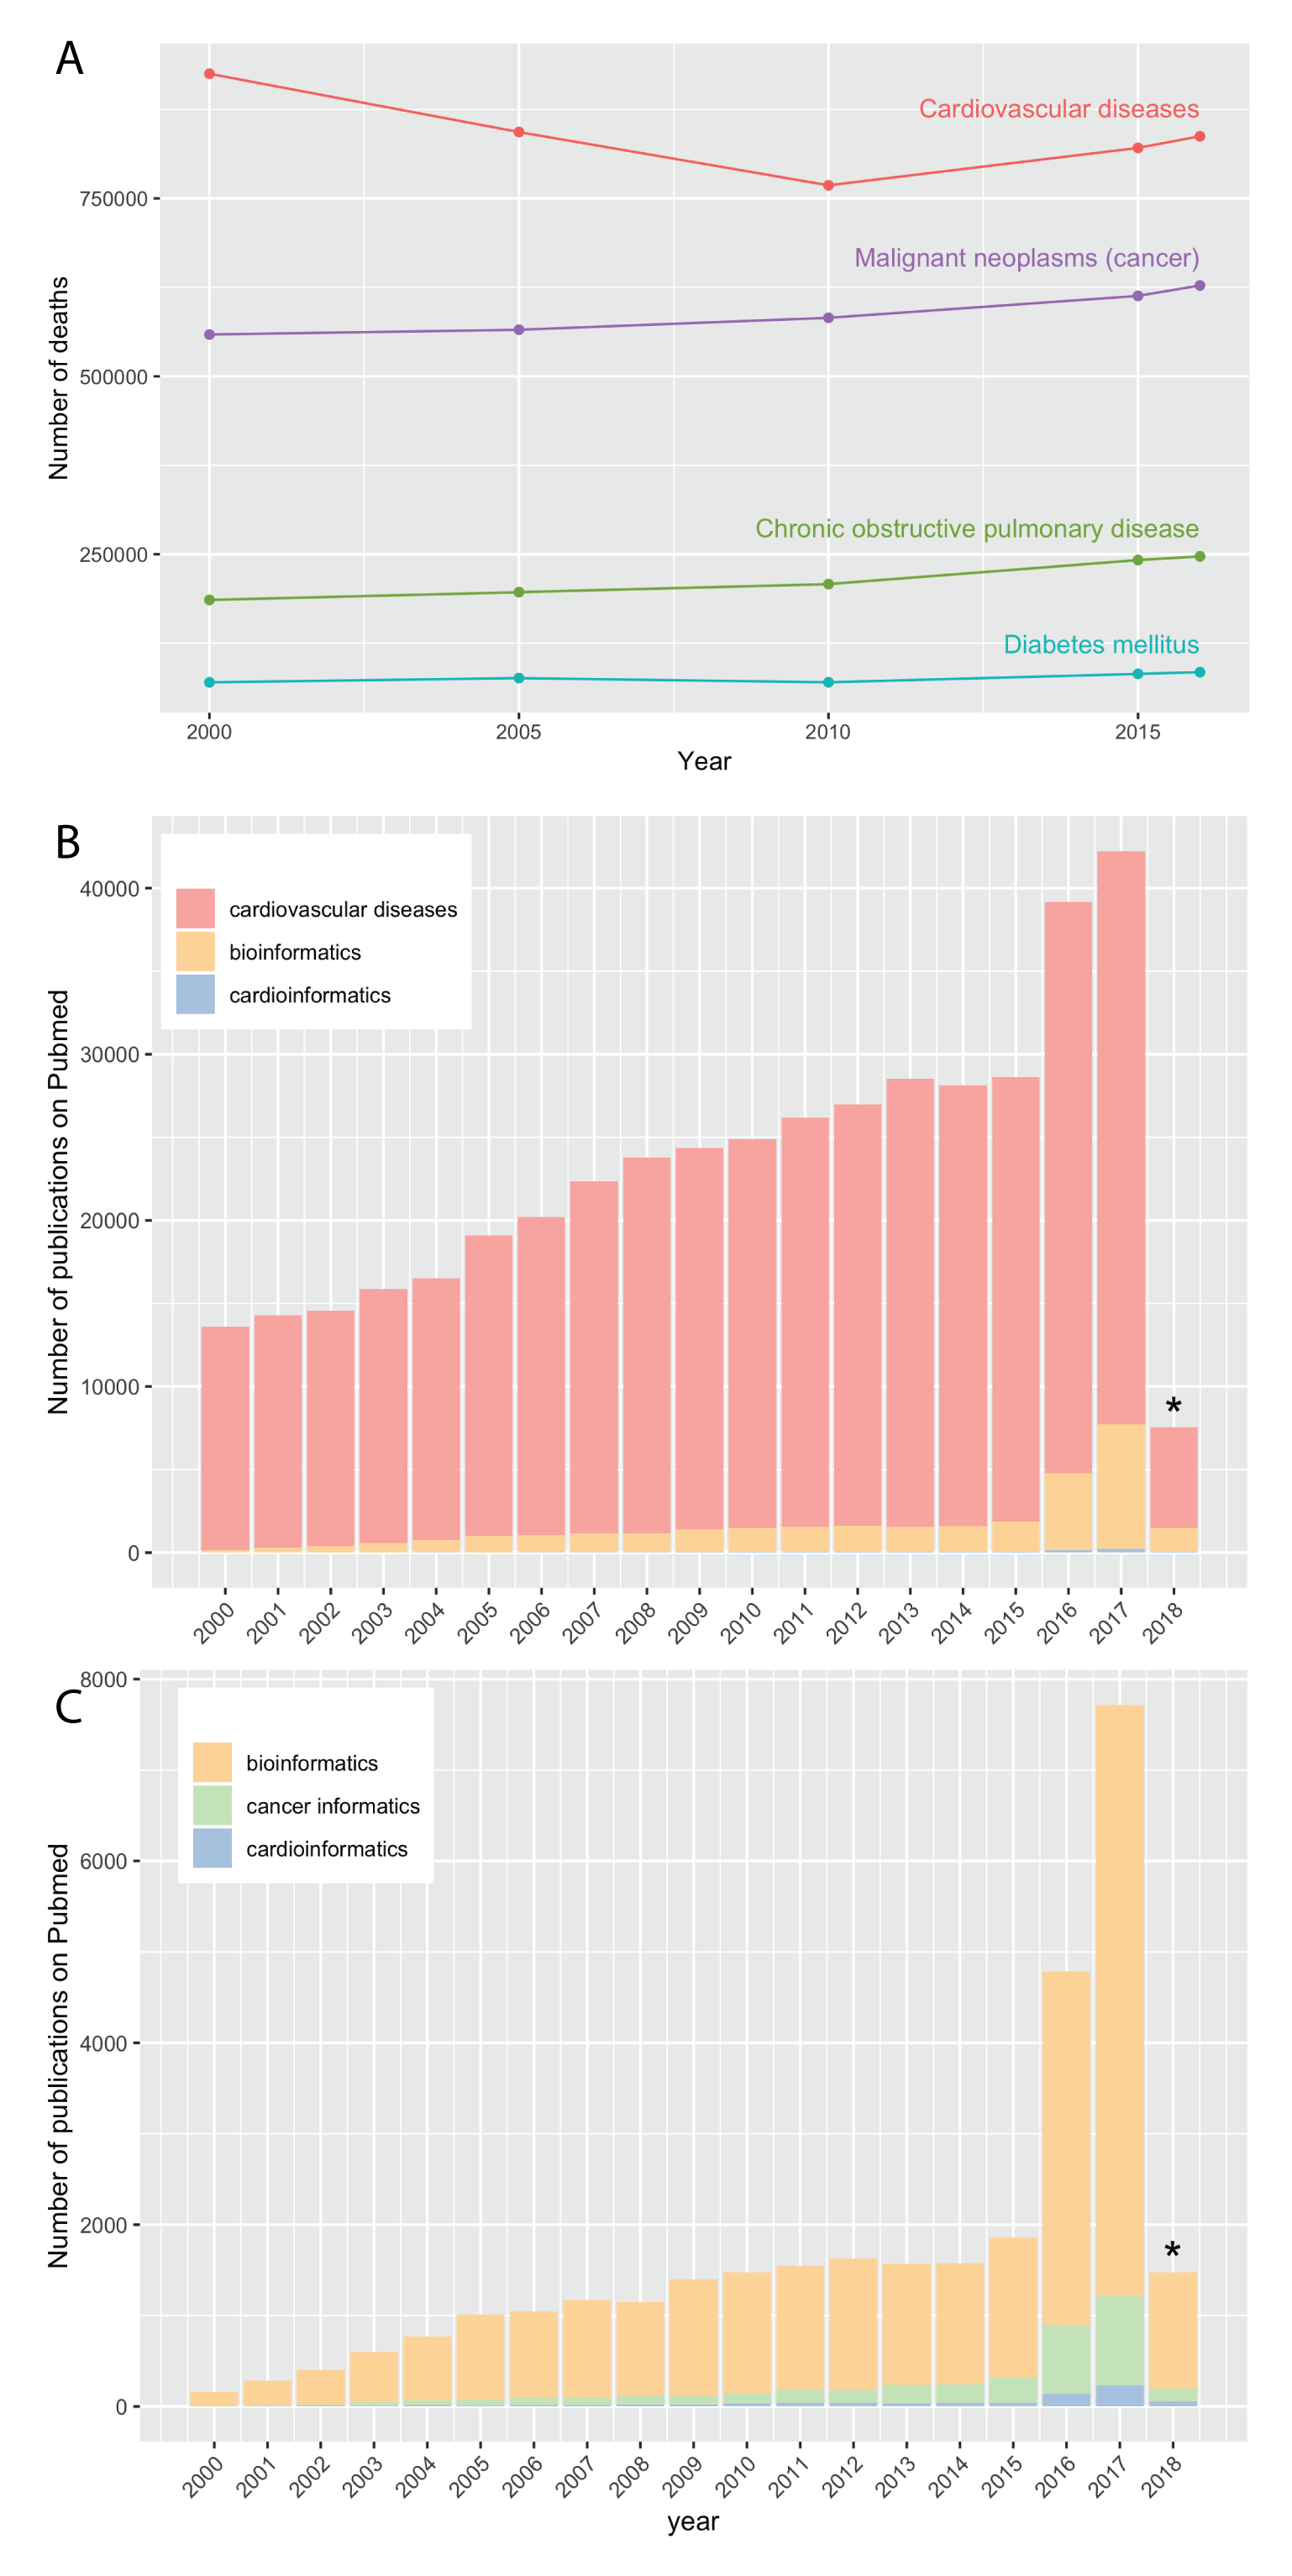
\includegraphics[width=1\linewidth]{figure1}
	\caption{\textbf{A}. Number of deaths by Non-Communicable Diseases in the US. \textbf{B}. \textbf{C}.}
	\label{fig:figure1}
\end{figure}

Cardiovascular diseases (CVD) have been persistently the leading cause of deaths by non-communicable diseases in the US for the last two decades (Figure \ref{fig:figure1}A). CVD research has steadily increased since 2000, resulting in an immense body of publications indexed in PubMed. In 2017 alone, there are more than 40000 articles classified with the subject heading "cardiovascular disease" (defined according to the Medical Subject Heading -- MeSH terms), not including reviews. (The MeSH Database entry for \textit{cardiovascular disease} includes many types of cardiovascular abnormalities which may occur in organs other than the circulatory system.) Among these outputs, the share of bioinformatics research remains modest, almost invisible. Despite the being present in the current tide of precision medicine initiatives, cardiovascular research is critically lacking in bioinformatics which play a critical role in precision medicine \citep{Gomez-Lopez:2017:Precision}.  The modest contribution of bioinformatics in cardiology is in stark contrast to that in cancer, to some extent suggesting that there are ample opportunities for cardioinformatics. In this review, we highlight the contemporary problems in the research of CVD genetics, introduce the bountiful resources available and propose the ways to advance this field and leverage cardiovascular research with bioinformatics.

The first draft of the human genome project had brought a lot of hope and excitement about potential advancements in the diagnosis and treatment of cardiac diseases, such as the ability to identify disease genes within the associated loci, to improve risk estimation based on more precise genotypes, or to personalize the prediction of drug effect on a patient, \citep{Komajda:2001:heart}.

%{https://www.ncbi.nlm.nih.gov/mesh/68002318} 


\section{Complexity of CVDs}

\subsection{The increasing number of actors}

As more studies are published, the number of genes involved in a disease has also increased and in most cases, gone beyond a few genes that could be described in a single-page table or diagram.


As the most common cause of heart transplantation, dilated cardiomyopathy (DCM) worths investigating. In a recent review \citep{Burke:2016:Clinical} 16 disease-causing genes were compiled, along with an additional 41 putative genes. Meanwhile, GWAS catalog and HPO annotation suggested a much larger number of genes associated with this condition, 69 genes and 115 genes, respectively. These numbers clearly advocate for more bioinformatics analyses to gain insights into this condition and the other conditions that are equivalently complex.

According the amount of possible interactions between them increase combinatorially.

Accordingly, the number of biological states is exponential. Among these states, it is obvious that biological systems do not seek for a single optimal state, but always strive for the most convenient functional one. Therefore, it is reasonable to expect a diverse set of states in which biological system is equivalently functional.

As with other complex diseases, missing heritability has been a long-standing puzzle in cardiovascular diseases \citep{Manolio:2009:Finding}. Despite the early successes in pinpointing the causes of several monogenic diseases, the large body of genome-wide association (GWA) studies have defied many widely held beliefs about genetic variants in human, hinting at the directions to search for the missing heritability.

polygenic score: how many genes involved




rare variants

The most trivial situation where inherited risk is not fully accounted for is when the variants are simply too rare to be detected with sufficient power. One addresses this issue by collecting more samples or improving statistical tests.

The availability of a large number of genomes and exomes, on one hand enabled the detection of such rare variants, and on the others,  showed that rare variants 


\subsection{The under-explored territories}

structural variants

An obvious reason for missing the significant variants is to search in the wrong place. Most genotyping arrays were designed to detect SNPs, essentially ignoring the structural variants including copy number variants, inversion, translocation, etc. As next-generation sequencing is employed in genotyping, the protein-coding part of the genome, i.e. \textit{exome} are prioritized, based on a regularly cited fact that the exome harbors 85\% of the disease-causing variants turns out to be an outdated estimate from 1995 \citep{Antonarakis:2001:nature}. Our survey of the variants having significant association with human traits, as compiled by GWAS (to limit to associations with p-value less than $10^{-5}$), revealed a large fraction in non-protein coding regions such as intron, interngenic, 5'-UTR, 3'-UTR, etc (Figure \ref{fig:variant_context}). Notably, the distribution of CVD-associated variants in the genome mimic that of the complete set of variants. This observation emphasizes the fact that our understanding of CVD as well as biology in general has been critically limited by our technical capability to characterize protein-coding genes. 


non-coding

epigenetics

What is epigenetics? 
Recent findings have unraveled a more important role of non-coding RNAs and epigenetics in cardiovascular biology.

environment interactions

A critical limitation to study at the molecular level is the interaction between gene  and environment.

It has been known for decades that non-genetic factors play a critical role in cardiovascular health, such that a risk prediction using lifestyle variables perform much better than a polygenic score \citep{Joyner:2011:Ten}. The understanding of this interaction at the molecular level is still relevant for basic research, as well as health care applications. The research has been limited due to the difficulties in monitoring one's external environment. Such barrriers start to be lifted, thanks to the development of wearable devices that can collect real time data in a non-intrusive manner. Studies on the exposome have started to accumulate \citep{Jiang:2018:Dynamic}, projecting the greater need of large scale, streaming data analysis.


\subsection{The forgotten concepts}

homeostasis

omnigenic model remind us about the widespread interactions possible in a cell and how important it is to account for most of the actors


\begin{figure*}[!tpb]
	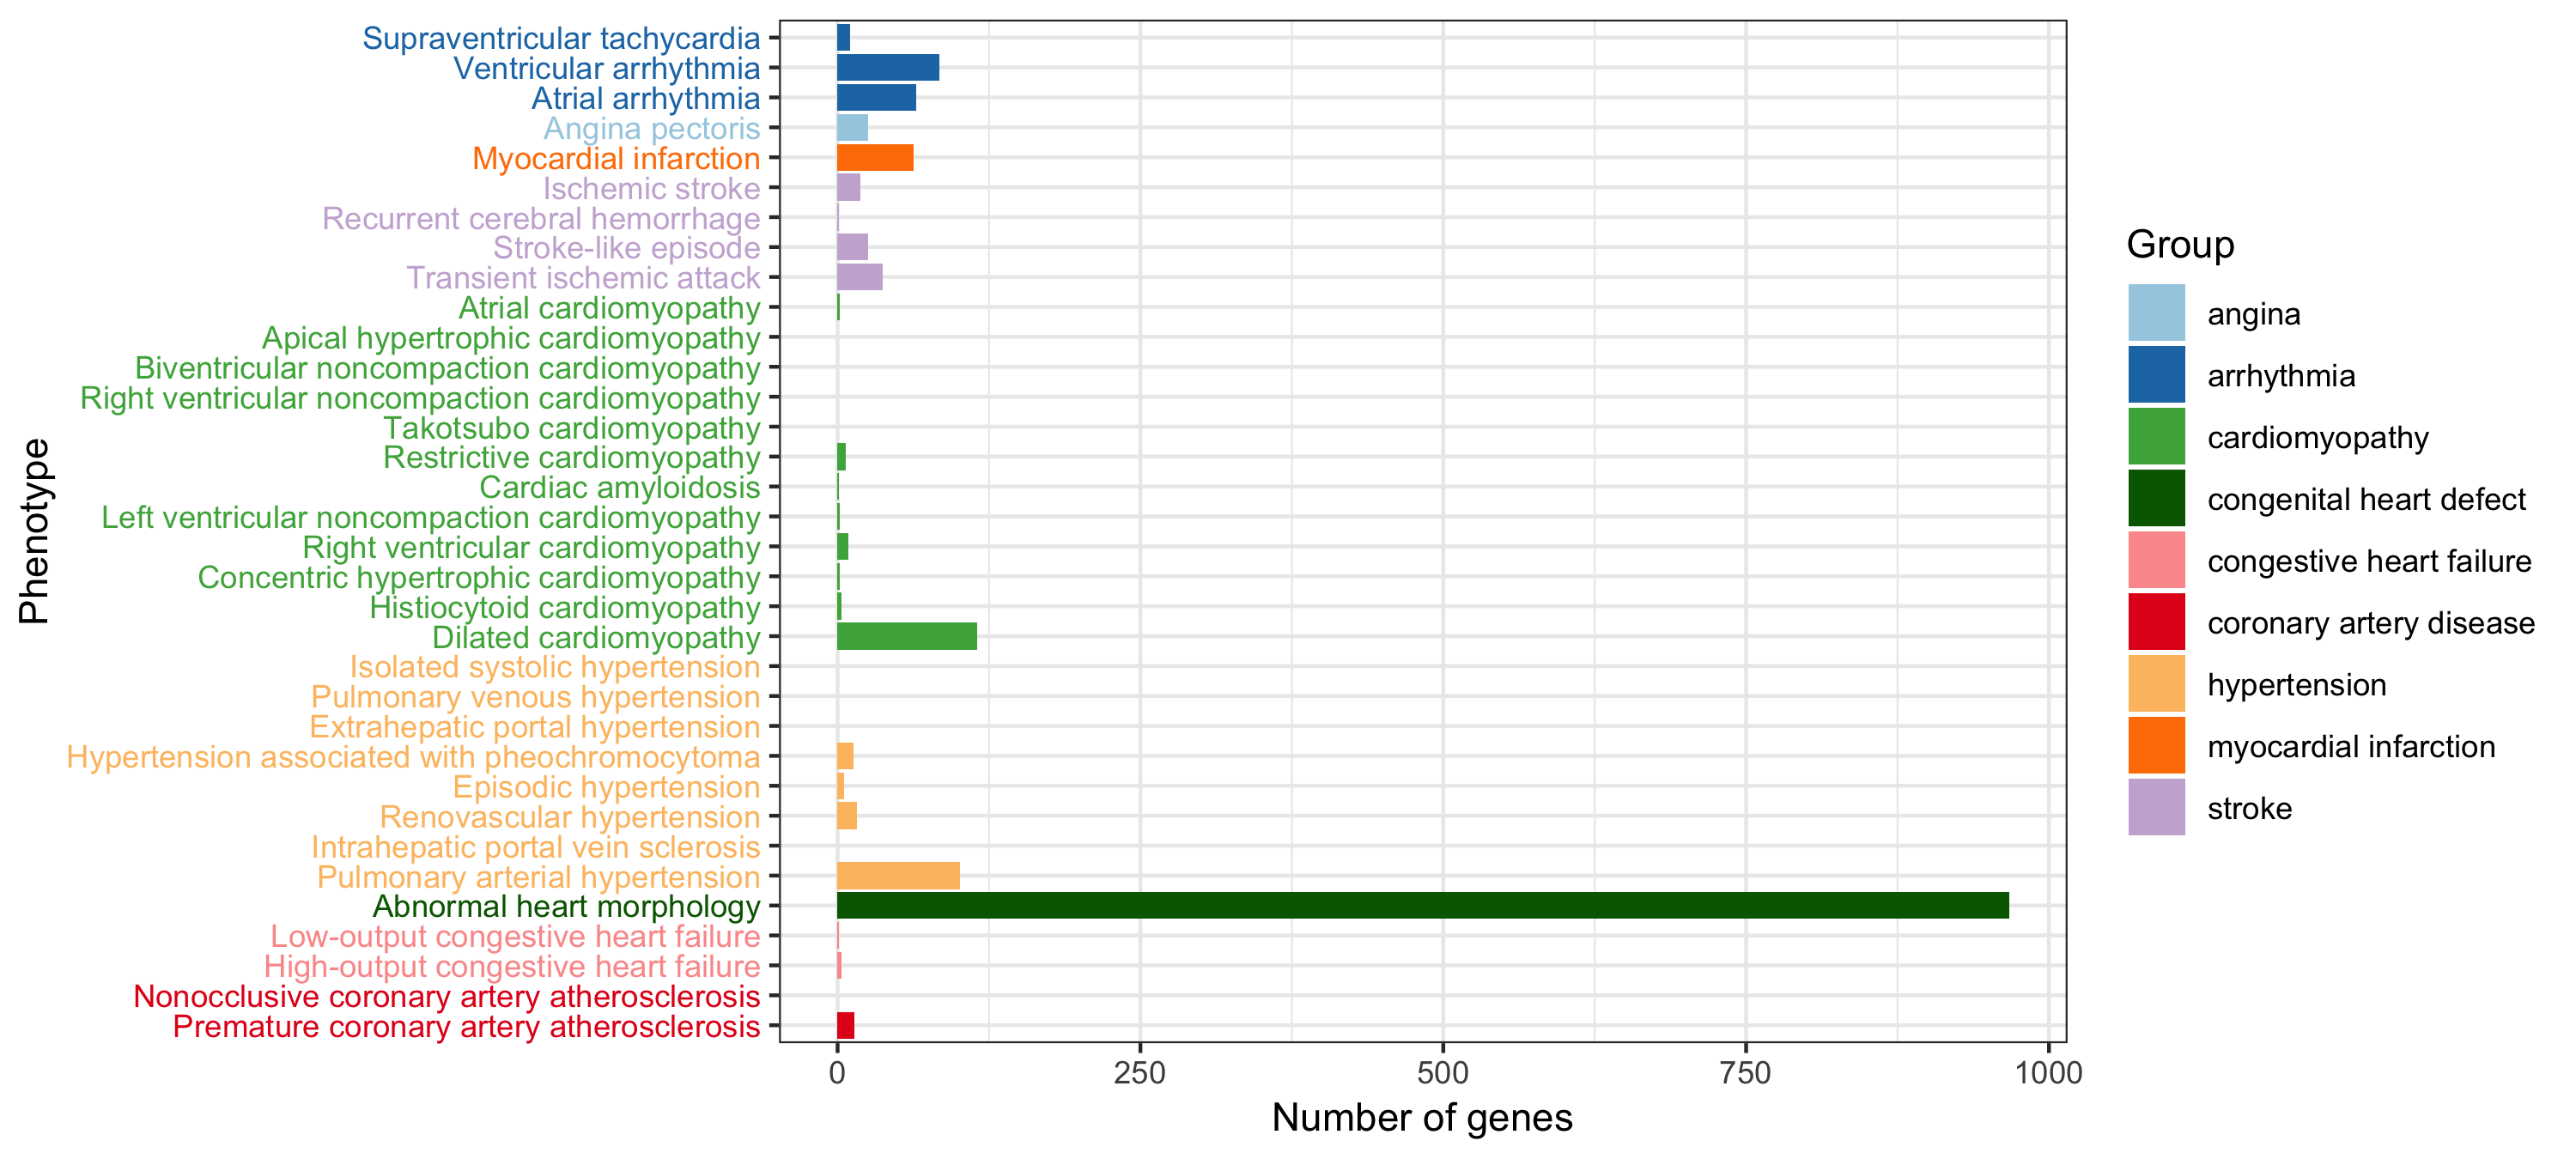
\includegraphics[width=1.\linewidth]{hpo-gene-count}
	\caption{The number of genes associated with \textit{Abnormality of the cardiovascular system} (HP:0001626) as annotated with the Human Phenotype Ontology \citep{Kohler:2014:Human}.}
	\label{fig:hpo_gene_count}	
\end{figure*}

\begin{figure}[!tpb]
	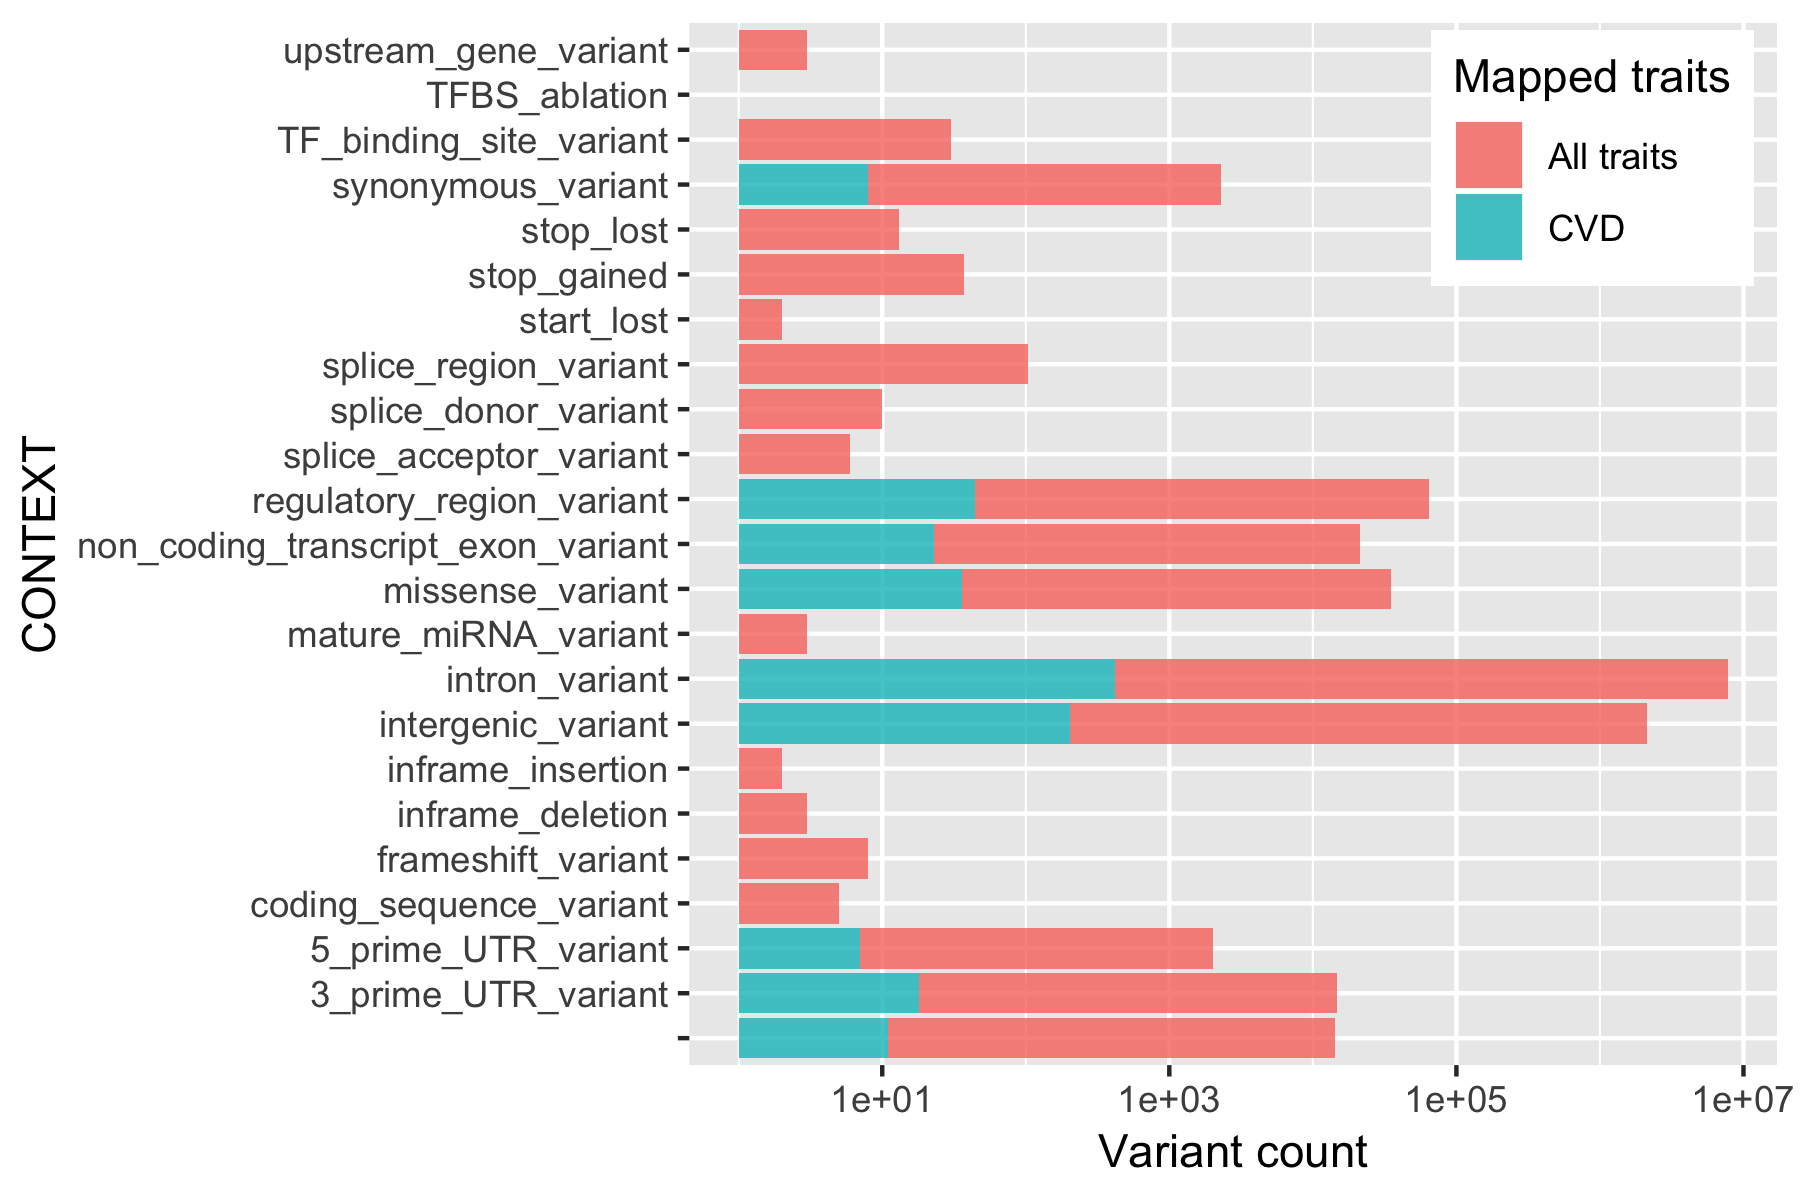
\includegraphics[width=1\linewidth]{variant_contexts_sigVars}
	\caption{Distribution of known variants in the human genome.}
	\label{fig:variant_context}
\end{figure}

%Some quantity showing the associations of CVD with genes...
%
Text Text Text Text Text Text  Text TextText Text Text Text Text Text  Text TextText Text Text Text Text Text  Text TextText Text Text Text Text Text  Text TextText Text Text Text Text Text  Text Text Text Text Text Text Text Text  Text Text Text Text Text Text Text Text  Text Text Text Text Text Text Text Text  Text Text Text Text Text Text Text Text  Text Text Text Text Text Text Text Text  Text Text Text Text Text Text Text Text  Text Text Text Text Text Text Text Text  Text Text Text Text Text Text Text Text  Text Text Text Text Text Text Text Text  Text Text Text Text Text Text Text Text  Text Text Text Text Text Text Text Text  Text Text Text Text Text Text Text Text  Text Text Text Text Text Text Text Text  Text Text Text Text Text Text Text Text  Text Text Text Text Text Text Text Text  Text Text Text Text Text Text Text Text  Text Text Text Text Text Text Text Text  Text Text Text Text Text Text Text Text  Text Text Text Text Text Text Text Text  Text Text Text Text Text Text Text Text  Text Text Text Text Text Text Text Text  Text Text Text Text Text Text Text Text  Text Text Text Text Text Text Text Text  Text Text Text Text Text Text Text Text  Text Text Text Text Text Text Text Text  Text Text 

Text Text Text Text Text Text  Text Text Text Text Text Text Text Text  Text Text Text Text Text Text Text Text  Text Text Text Text Text Text Text Text  Text Text Text Text Text Text Text Text  Text Text Text Text Text Text Text Text  Text Text Text Text Text Text Text Text  Text Text Text Text Text Text Text Text  Text Text Text Text Text Text Text Text  Text Text Text Text Text Text Text Text  Text Text Text Text Text Text Text Text  Text Text Text Text Text Text Text Text  Text Text Text Text Text Text Text Text  Text Text Text Text Text Text Text Text  Text Text Text Text Text Text Text Text  Text Text Text Text Text Text Text Text  Text Text Text Text Text Text Text Text  Text Text Text Text Text Text Text Text  Text Text Text Text Text Text Text Text  Text Text Text Text Text Text Text Text  Text Text Text Text Text Text Text Text  Text Text Text Text Text Text Text Text  Text Text Text Text Text Text Text Text  Text Text Text Text Text Text Text Text  Text Text Text Text Text Text Text Text  Text Text Text Text Text Text Text Text  Text Text Text Text Text Text Text Text  Text Text Text Text Text Text Text Text  Text Text Text Text Text Text Text Text  Text Text Text Text Text Text Text Text  Text Text Text Text Text Text Text Text  Text Text Text Text Text Text Text Text  Text Text Text Text Text Text Text Text  Text Text Text Text Text Text Text Text  Text Text Text Text Text Text Text Text  Text Text Text Text Text Text Text Text  Text Text Text Text Text Text Text Text  Text Text Text Text Text Text Text Text  Text Text Text Text Text Text Text Text  Text Text  


%
\section{Cardioinformatics}
%%

\subsection{The soil is worked}

This part is to introduce the achievements and on-going work in developing the infrastructure for data storage, management and sharing, thus making the case for an invest in bioinformatics analyses to capitalize on these resources.


\subsubsection{Infrastructure}

The infrastructure for bioinformatics analyses now is even more mature, thanks to cloud computing \citep{Langmead:2018:Cloud}, secured data storage and management.

Guidelines, protocol


Text Text Text Text Text Text  Text Text Text Text Text Text Text Text  Text Text Text Text Text Text Text Text  Text Text Text Text Text Text Text Text  Text Text Text Text Text Text Text Text  Text Text Text Text Text Text Text Text  Text Text Text Text Text Text Text Text  Text Text Text Text Text Text Text Text  Text Text Text Text Text Text Text Text  Text Text Text Text Text Text Text Text  Text Text Text Text Text Text Text Text  Text Text Text Text Text Text Text Text  Text Text Text Text Text Text Text Text  Text Text Text Text Text Text Text Text  Text Text Text Text Text Text Text Text  Text Text Text Text Text Text Text Text  Text Text Text Text Text Text Text Text  Text Text Text Text Text Text Text Text  Text Text Text Text Text Text Text Text  Text Text Text Text Text Text Text Text  Text Text Text Text Text Text Text Text  Text Text Text Text Text Text Text Text  Text Text Text Text Text Text Text Text  Text Text Text Text Text Text Text Text  Text Text Text Text Text Text Text Text  Text Text Text Text Text Text Text Text  Text Text Text Text Text Text Text Text  Text Text Text Text Text Text Text Text  Text Text Text Text Text Text Text Text  Text Text Text Text Text Text Text Text  Text Text Text Text Text Text Text Text  Text Text Text Text Text Text Text Text  Text Text Text Text Text Text Text Text  Text Text Text Text Text Text Text Text  Text Text Text Text Text Text Text Text  Text Text Text Text Text Text Text Text  Text Text Text Text Text Text Text Text  Text Text Text Text Text Text Text Text  Text Text Text Text Text Text Text Text  Text Text 

\subsubsection{Profusion of data}

Technological advances brought about the accumulation of biological data, both in the number of data points, and the number of dimensions in each data point.
High-throughput profiling techniques are inarguably the main drive in creating high-dimensional data (DNA, RNA, protein levels).
A glimpse into central repositories such as GEO or dbGaP hinted at the amount of data points that can be accumulated from small  studies. Depending on the questions at hands, the precise definition of a data point can vary. In most cases, it can be equivalent to the number biological samples or that of individual donors. Although studies directly related to CVDs are of interest when it comes to future CVD research, a significant number of data points from non-CVD studies can be put into use, for example, when these studies investigated samples of cardiovascular origin (heart or vascular tissues).

\begin{figure}[!tpb]%figure1
	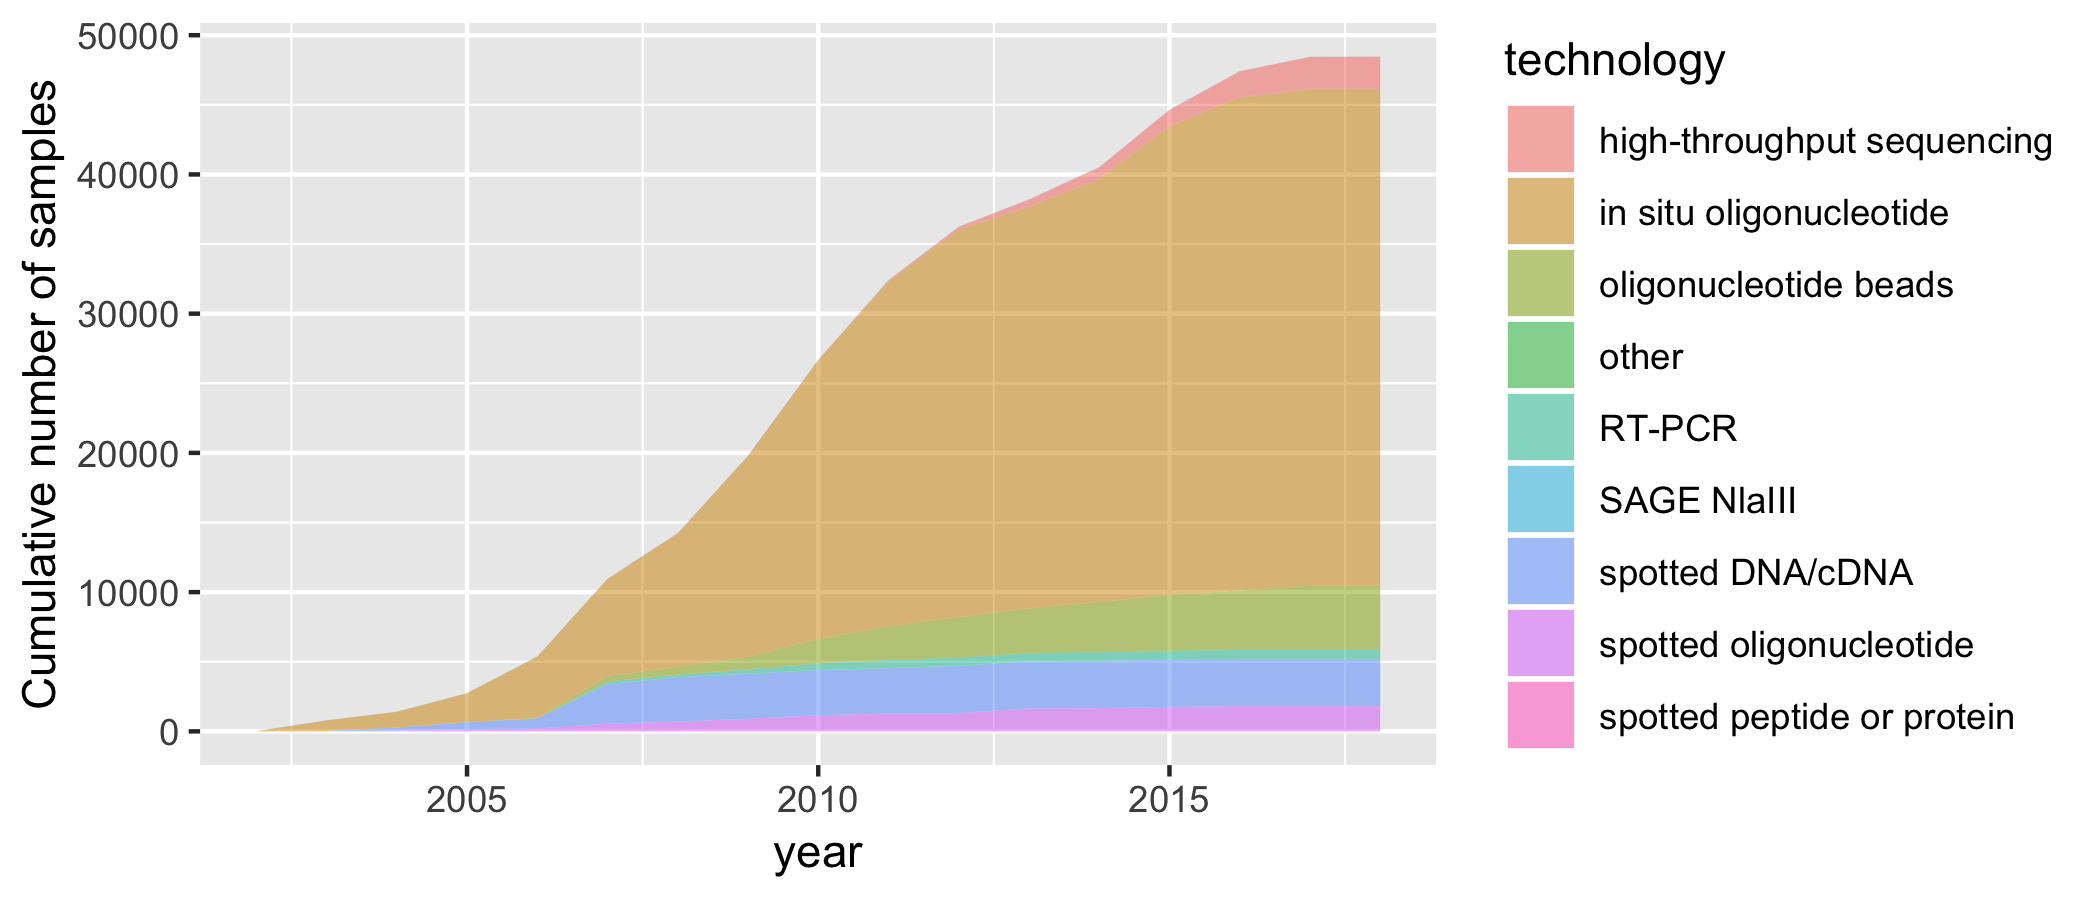
\includegraphics[width=1\linewidth]{gsm_count_by_tech.png}
	\caption{The cumulative number of samples deposited on GEO.}
	\label{fig:01}
\end{figure}

\begin{table}[!t]
	\processtable{Number of samples available on GEO that are of potential use of cardioinformatics research, including those deposited by CVD studies and non-CVD studies.\label{tab:geoSamples}} {\begin{tabular}{@{}llll@{}}\toprule 
			molecule &non-CVD studies & CVD studies \\ \midrule
			genomic DNA &            440 &        8525  \\
			polyA RNA &             89 &         392  \\
			total RNA &           2974 &       39540  \\
			other &             NA &           5  \\
			protein &             NA &           3  \\ \botrule
	\end{tabular}}{This is a footnote}
\end{table}

The figures given in Table \ref{tab:dbgapSubject} are in fact conservative estimates of the data generated so far among the research community. A much larger amount of data are stored on dbGaP and accessible upon approval of data request. Among these, the number of subjects involved in CVD research alone are more than 600000. %658305 to be exact

\todo{supplement table if necessary}

Aside from central authoritative repositories of research data, smaller databases with narrower focus are budding. For example, many databases have been created to collect chromatin structure data from 3C, 4C, 5C and HiC-seq experiments. A few databases are actively gathering knowledge about non-coding RNAs. Being in these under-explored territories, researchers may need more work to collect and curate their data from multiple sources before using them for further analyses.

% Please add the following required packages to your document preamble:
% \usepackage{booktabs}
\begin{table}[]
	\caption{The subject count aggregated from studies deposited in dbGaP, licensed for General Research Use}
	\label{tab:dbgapSubject}
	\begin{tabular}{l l l}
		\toprule
		& \textbf{CVD} &  \textbf{All}                         \\ \midrule
		16s rRNA (NGS)                 &     0 &      92 \\
		CNV Genotypes                  &     0 &   48972 \\
		Chromatin (NGS)                &     0 &     139 \\
		Genomic Sequence Amplicon (NGS)&     0 &       8 \\
		Methylation (CpG)              &     0 &     657 \\
		Methylome sequencing           &     0 &     152 \\
		QTL Results                    &     0 &     281 \\
		RNA Seq (NGS)                  &   333 &    1498 \\
		SNP Genotypes (Array)          &  6658 &  113597 \\
		SNP Genotypes (NGS)            &  4277 &   11786 \\
		SNP Genotypes (PCR)            &     0 &      10 \\
		SNP Genotypes (imputed)        &     0 &   29693 \\
		SNP/CNV Genotypes (NGS)        &     0 &     936 \\
		SNP/CNV Genotypes (imputed)    &     0 &    9291 \\
		SNV (.MAF)                     &     0 &       2 \\
		SNV Aggregate (.MAF)           &     0 &     570 \\
		Targeted Genome (NGS)          &     0 &    9918 \\
		Whole Exome (NGS)              &  5518 &   12771 \\
		Whole Genome (NGS)             &     0 &    1245 \\
		mRNA Expression (Array)        &     0 &     798 \\
		miRNA (NGS)                        & 0 &   228 \\ \hline
	\end{tabular}
\end{table}

Text Text Text Text Text Text  Text Text Text Text Text Text Text Text  Text Text Text Text Text Text Text Text  Text Text Text Text Text Text Text Text  Text Text Text Text Text Text Text Text  Text Text Text Text Text Text Text Text  Text Text Text Text Text Text Text Text  Text Text Text Text Text Text Text Text  Text Text Text Text Text Text Text Text  Text Text Text Text Text Text Text Text  Text Text Text Text Text Text Text Text  Text Text Text Text Text Text Text Text  Text Text Text Text Text Text Text Text  Text Text Text Text Text Text Text Text  Text Text Text Text Text Text Text Text  Text Text Text Text Text Text Text Text  Text Text Text Text Text Text Text Text  Text Text Text Text Text Text Text Text  Text Text Text Text Text Text Text Text  Text Text Text Text Text Text Text Text  Text Text Text Text Text Text Text Text  Text Text Text Text Text Text Text Text  Text Text Text Text Text Text Text Text  Text Text 

%
%\subsubsection{Basic research}
%for data management, computational analysis, visual representation, etc.
%
%\subsubsection{Clinical application}
%
%

\subsection{Computational methods}

As early as 1999 when the complete human genome and high-throughput transcriptomic profiling are on the horizon, research community have started to recognize the critical use of bioinformatics analyses in generating insights from these data. The computational approaches outlined by \cite{Claverie:1999:Computational} for the early day gene expression data are still popular in today transcriptomics studies: differential gene expression analysis, co-expression analysis and gene clustering with subsequent identification of enriched biological pathways. Those old-fashioned methods can still bring fruitful analyses, as illustrated in a recent study on heart failure \citep{Santolini:2018:personalized}.

The application of machine learning will be indispensable in many aspects of cardiology \citep{Shameer:2017:Translational,Shameer:2018:Machine}. Given the availability of machine learning performant implementations, cardioinformatics is better positioned to tackle domain-specific questions and develop clinical application. For example, ML can be applied to enhance medical image. In basic research, natural language processing can be a promising tool to improve data collection and organization.


With less focus on computation, visualization still makes up an important part in facilitating biological research, especially for data exploration, pattern recognition, and data representation. Visualization methods are blooming to accommodate the diverse data types in biology \citep{Pavlopoulos:2015:Visualizing}. With regard to visualization, the exciting challenge to cardioinformatics researcher is the meaningful integrated representation of data layers. In basic research, such representation can mean to put together pieces of information from various experimental techniques. In clinical application, the focus is on facilitating clinical decisions.

Search engine and knowledge synthesis \citep{Lutjohann:2011:Sciencenet}.

%\subsection{The multi-layered paths from genome to phenotype}

This part is to demonstrate the volume of existing data and the potential of new insights from re-analyses, especially when more than one layers are stacked. Give the examples of those multi-omics studies.


\todo{Tentative: A figure/table enlisting layers of modifications that contribute to determine a phenotype, with the corresponding experimental techniques}

\cite{Santolini:2018:personalized} 

\cite{Klarin:2017:Genetic}


%%
%\begin{itemize}
%	\item genome
%	\item epigenome
%	\item transcriptome: mRNA, non-coding RNA: microRNA, long non-coding RNA
%	\item 	proteome
%	\item	metabolome
%\end{itemize}
%%environmental factors
%
%

\subsection{New and re-newed perspectives}

Cardioinformatics offers a number of powerful concepts to investigate complex physiological system.

The paradigm shift from the physical genes to the "eigengenes" in studying complex diseases \citep{Weiss:2012:Good} is a pragmatic approach. This approach allows one to focus on mimicking the healthy system without the knowledge required to model the individual actors and their interactions, making it an ideal method in the drug discovery workflow. The paradigm can help advancing knowledge further because it suggests an efficient way to engineer biological system and learn how it works.

The heavily connected biological system is among many types that can be modeled and analyzed as graphs. The omnigenic model recently proposed has highlighted the need for this system-level modeling, since the involvement of peripheral genes are widespread in physiological and pathological processes.

\section{Conclusion}


%

\enlargethispage{12pt}




\section*{Acknowledgements}

Text Text Text Text Text Text  Text Text.  
\vspace*{-12pt}

\section*{Funding}

This work has been supported by the... Text Text  Text Text.\vspace*{-12pt}

\bibliographystyle{natbib}
%\bibliographystyle{achemnat}
%\bibliographystyle{plainnat}
%\bibliographystyle{abbrv}
%
%\bibliographystyle{plain}
%
\bibliography{cardio}



\end{document}
